\chapter{外文资料的调研阅读报告或书面翻译}

\title{城市道路自动驾驶车辆运动计划和控制研究综述}

{\heiti 摘要:} 自动驾驶车是一种成熟的技术,通过提高汽车运输的安全性,可及性,效率和便利性,有可能重塑人们的出行方式。 自驾车必须在确保安全的前提下执行任务,包括通过与其他车辆和行人共享的动态环境进行动作规划,以及通过反馈控制可靠地执行动作。 本文的目的是调查目前的规划和控制算法的现状,特别是在城市环境中。本文对部分所提出的技术进行了综述,并讨论了其有效性。 所调查的方法在所使用的车辆移动性模型,环境结构假设和计算要求方面不同。 本次调查中的并列比较有助于深入了解经过调查的方法的优势和局限性,并辅助系统级设计选择。

\section*{A.1\ \ 介绍}

过去三十年来,学术界和工业界都在不断开展无人驾驶技术的研究工作。传感和计算技术的最新进展,无人驾驶技术对汽车运输的潜在转变及其社会效益,推动了这项技术的发展:2014年有交通相关死亡人员32,675人,其中230万人受伤,610万起交通事故被报道[1]。其中,估计有94\%的事故是由驾驶员操作失误造成,31\%涉及饮酒的驾驶员,10\%涉及分心的驾驶员[2]。自动驾驶车有可能大大减少因驾驶员犯错和疏忽而造成的事故。它们还将为由于身体或视觉残疾而无法驾驶的人提供私人交通工具。最后,全美工作人口86\%的人每天平均花25分钟(单程)的时间乘汽车上下班,自动驾驶车将有助于更有效地利用通勤时间,或简单地减少驾驶压力带来的不良影响[4]。

考虑到这种新技术的潜在影响,自驾车已经有悠久的历史。这个想法早在20世纪20年代就已经存在,但直到20世纪80年代,无人驾驶的汽车才真正成为可能。 20世纪80年代由恩斯特·迪克曼(Ernst Dickmanns)(例如[5])领导的开创性工作为无人车的开发铺平了道路。那时候,PROMETHEUS项目的大量研究力量投入了无人车的研发。 1994年,由VaMP开发的无人驾驶汽车驾驶1600公里,其中95\%是自主驾驶[6]。在同一时期,CMU NAVLAB正在该领域取得进展,并在1995年展示了进一步的进展,在5000公里穿越美国的车程中,98\%是自主驾驶[7]。

无人驾驶汽车技术的下一个重大里程碑是2004年第一次DARPA大挑战赛。比赛目标是让无人驾驶汽车尽快通过150英里的越野赛道。与以前的展示相比,这是一个重大的挑战,因为在比赛中不会有人为的干预。虽然以前的工作能实现几乎自主的驾驶,但在关键时刻消除人为干预被证明是一个重大的挑战。15辆车中没有一辆完成比赛。 2005年举办了类似的活动;这一次,23支队伍中有5个到达了终点线[8]。后来,2007年,DARPA城市挑战赛举行,车辆被要求在模拟城市环境中自主驾驶。六个小组完成了这一比赛,表明完全自主的城市驾驶是可能的[9]。

自从DARPA挑战以来,全世界已经进行了许多比赛和较大的无人车系统测试。值得注意的例子包括2009年至2013年的智能车辆未来挑战赛[10],2010年的现代汽车无人车挑战赛[11],2010年的VisLab洲际无人车挑战赛[12],2013年的城市无人驾驶汽车公路测试[13],以及Bertha-Benz路线的自主驾驶测试[14]。同时,在学术环境的改善和行业发展的驱动下,无人车研究工作进展顺利。 Google自驾车[15]和特斯拉的自动驾驶仪系统[16]是获得广泛关注的商业活动的两个例子。

汽车自动化的程度可以从完全由人操作到完全自主操作。 SAE J3016标准[17]引入了从0到5的等级分级车辆自动化程度。在这个标准中,0级代表车辆所有驾驶任务都是人类驾驶员完成。1级包括基本驾驶辅助,如自适应巡航控制,防抱死制动系统和电子稳定控制[18]。2级包括高级辅助系统,如危害最小化纵向/横向控制[19]和紧急制动[20],[21],这些系统通常基于预先设定形式的控制理论来计算“最坏情况” (安全)状态[22] - [24],确保车辆无碰撞。在3级系统中,系统对行车环境进行监控,并且可以在某些条件下完全自主地运行,但如果驾驶任务离开自主系统的操作范围,则仍然需要操作人员进行控制。具有4级自动化的车辆能够在某些条件下完全自主驾驶,并且如果操作者没有根据要求进行干预,仍可以安全地控制车辆。 5级系统在所有驾驶模式下都是完全自主的。

车载计算和无线通信技术的可用性允许汽车与其他车辆和道路基础设施交换信息,引发了与之密切相关的智能网联车技术的研究[25]。这方面研究旨在通过个别车辆之间的信息共享和协调来提高道路运输的安全性和性能。例如,网联车技术有可能改善交叉点处的吞吐量[26]或阻止交通冲击波的形成[27]。

为了限制本次调查的范围,我们专注于自主驾驶汽车的决策,运动规划和控制方面,特别是对于3级及以上的自动化系统。出于同样的原因,自动驾驶车的感知技术被忽略,读者可以参考关于这一主题的一些综述和近期的重要进展[28] - [31]。

当代自主驾驶系统的决策通常分层次地组织成路线规划,行为决策,局部运动规划和反馈控制。然而,文献中有许多不同的划分,因此对决策级别的划分相当模糊。本文对于解决这些自主驾驶核心问题所提出的方法展开了调查,特别强调局部运动规划和控制的方法。

本文的其余部分结构如下:第二部分对决策过程层次进行了概述,展示了部分设计方法。第三节回顾了用于在城市环境中估计汽车的移动性的模型,以便进行运动规划和反馈控制的研究。第四节调查有关运动规划的丰富文献,并讨论其对自驾车的适用性。同样,第五节讨论了无人驾驶汽车的路径和轨迹稳定问题以及具体的反馈控制方法。最后,第六部分总结了并评述了研究现状和未来研究方向。


\section*{A.2\ \ 无人车决策层次概述}

在本节中,我们将描述典型自驾车的决策层次,并对每个部分的功能进行描述。无人驾驶汽车本质上是自动决策系统,可处理来自车载传感器(如雷达,LIDAR,摄像机,GPS / INS单元和测距仪)的观测数据流。这些观察结果以及关于道路网络的现有知识,道路规则,车辆动力学和传感器模型被用于自动选择控制车辆运动的控制变量的值。智能车辆研究旨在尽可能多地自动化驾驶任务。该问题通常采用的方法是将感知和决策任务分解和组织成一个层次结构。感知系统使用先前的信息和收集的观测数据来提供车辆状态及对周围环境的估计,然后由决策系统使用估计来控制车辆,从而完成驾驶目标。

典型自驾车的决策系统被分层分解为四个组成部分(参见图\ref{fig:decision}):在最高层,路线是通过道路网计划的。这之后是一个行为层,决定了一个局部的驾驶任务,逐渐将汽车导向目的地,并兼顾交通规则。运动规划模块然后在通行环境中规划一条连续路径以完成局部导航任务。最后由控制系统在运动的执行中反馈性地纠正错误。在本节的其余部分,我们将更详细地讨论每个部分的功能。

\begin{figure}
\centering
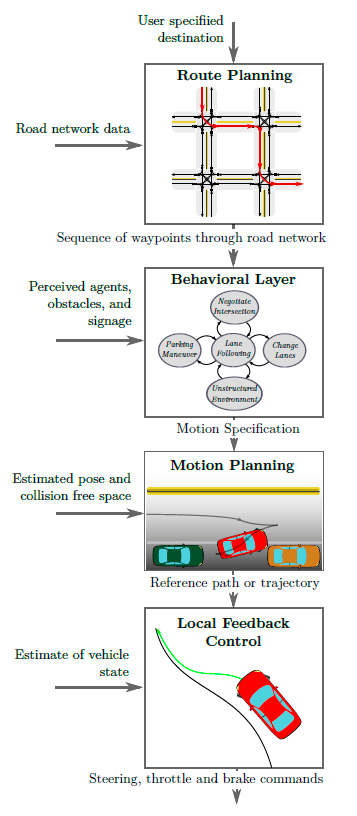
\includegraphics[width=8cm]{decision.png}
\captionsetup{margin=2cm}
\caption{无人车决策层级图}
\caption*{目的地作为路径规划层的输入,生成路网上的路径。行为决策层根据该路径和周围环境,生成一列指向目的地的具体行动。运动规划层进而规划出完成该行动的可行路径。反馈控制调整执行变量以纠正执行参考路径中的错误。}
\label{fig:decision}
\end{figure}

\subsection*{A.2.1\ \ 路径规划}
在最高级别,车辆的决策系统必须选择通过道路网从当前位置到所要求的目的地的路线。通过将道路网络表示为具有与穿越该路段的成本相对应的赋权有向图,可以将路径规划问题转化为在道路网络图上找到最小成本路径的问题。然而,代表道路网络的图形可以包含数百万条边,使得经典的最短路径算法(如Dijkstra [32]或A * [33])不切实际。运输网络中高效路线规划的问题引起了运输科学界的极大兴趣,研究者发明了一系列算法,经过一次性预处理步骤,可以在几毫秒内在大陆规模的网络上返回最佳路径[34],[35]。对于可用于有效规划驾驶员驾驶和自动驾驶车路线的实际算法的综合调查和比较,参见[36]。

\subsection*{A.2.2\ \ 行为决策}
在找到路线之后,无人车必须能够根据交通规则,导航所选择的路线,并与其他交通参与者进行交互。给定指示所选路线的路段的序列,行为决策层负责根据其他交通参与者的感知行为,路况和基础设施的信号在任意时间点选择合适的驾驶行为。例如,当车辆在交叉口前到达停车线时,行为层将命令车辆停下来,观察交叉路口处的其他车辆,自行车和行人的行为,并当轮到本车运行时发出运行指令。驾驶手册规定了具体驾驶环境的定性动作。由于驾驶环境和每个环境中可用的行为都可以被建模为有限集,自动化这种决策的自然方法是将每个行为建模成有限状态机中的状态,其中转移由感知到的驾驶环境控制,如本车相对于计划路线和附近车辆的位置。事实上,DARPA城市挑战中大多数团队都采用了有限状态机与特定于驾驶场景的不同启发式搜索[9]作为行为控制机制。

然而,现实世界的驾驶,特别是在城市中,其他交通参与者的意图不确定。研究者们还研究了其他车辆,自行车和行人未来轨迹的意图预测和估计问题。所提出的解决方案是基于机器学习的技术,例如高斯混合模型[37],高斯过程回归[38](这种方法被用于Google自主驾驶系统中意图预测的学习[39]),以及基于模型的直接从传感器测量数据估计意图的方法[40],[41]。

其他交通参与者的行为中的这种不确定性在行为决策层中通常建模为概率模型(例如马尔可夫决策过程(MDP))。例如,[42]在MDP框架中制定行为决策。一些工作[43] - [46]将未观察到的驾驶场景和行人意图显式建模为部分可观察的马尔可夫决策过程(POMDP),并提出具体的求近似解的策略。

\subsection*{A.2.3\ \ 运动规划}
当行为层决定在当前环境中执行的驾驶行为,例如跟驰,换道或右转时,所选择的行为必须被转换为路径或轨迹,才可以由低级反馈控制器跟踪。所得到的路径或轨迹必须对于车辆而言是动态可行的,对于乘客来说舒适,并且避免与车载传感器检测到的障碍物的碰撞。找到这样的路径或轨迹是运动规划系统的任务。

无人车的运动规划任务与机器人控制相关文献中讨论的求解标准运动规划的问题密切相关。在大多数情况下,运动规划问题的精确解决方案在计算上是不可行的。因此,在实践中通常使用数值近似方法。最常用的数值方法有变分法、图搜索发和增量树法等。其中变分法将轨迹求解问题转化为函数空间中的非线性优化问题;图搜索方法将构成车辆状态空间的道路拓扑图离散化并搜索最短路径;增量树法从车辆的初始状态逐渐构建可达状态树,然后选择这样一棵树的最佳分支。自动驾驶相关的运动规划方法在第四节中有更详细的讨论。

\subsection*{A.2.4\ \ 车辆控制}
为了执行运动规划系统确定的参考路径或轨迹,无人车使用反馈控制器来选择适当的执行器输入以执行计划的运动和纠正跟踪误差。 执行计划运动期间产生的跟踪误差部分原因在于车辆模型的不准确。 因此,闭环系统的鲁棒性和稳定性非常重要。

研究者们已经设计了许多有效的反馈控制器,来执行由运动规划系统提供的参考路径或轨迹。 相关技术在第五节中有详细的讨论。

\section*{A.3\ \ 无人车运动模型}
在本节中,我们将调查最常用的车辆运动模型。这些模型被广泛用于控制和运动规划算法中,来近似车辆的行为,响应相关操作条件下的控制动作。高保真模型可以准确反映车辆对控制量输入的响应,但是附加的细节可能使计划和控制问题复杂化。这提供了所选模型的准确性与决策问题的难度之间的权衡。本节概述了一般建模概念和运动规划和控制模型。

建模从车辆配置的概念开始,代表其在世界上的姿势或位置。例如,配置可以表示为汽车上的点与汽车的航向的平面坐标。这是汽车配置空间的坐标系。该坐标系描述平面刚体运动(由特殊欧几里德组在两维中表示,SE(2)),并且是常用的配置空间[47] - [49]。车辆运动的规划和调整必须在遵循所选模型引入的限制的前提下,完成驾驶任务。

\subsection*{A.3.1\ \ 单轨道运动学模型}
在实际使用的最基本模型中,汽车由两个通过刚性连杆连接的轮子组成,并被限制在一个平面上移动[48] - [52]。 假设车轮在与地面的接触点处不会滑动,而可以绕其旋转轴线自由旋转。 前轮具有附加的自由度,允许其绕垂直于运动平面的轴线旋转,以对转向进行建模。 该模型的这两个特征反映了大多数乘客在不同时前进的情况下不能进行横向位移的经验。 更正式地说,这种机动性的限制被称为非完整约束[47],[53]。 非完整约束被表示为对汽车运动的差分约束。 该表达式取决于坐标系的选择。 该模型的各种变种通常被称为类车机器人,自行车模型,运动模型或单轨道模型。

以下是用于配置的几个常用坐标系中差分约束的推导。 参考图\ref{fig:kinematics},矢量$p_r$和$p_f$表示后轮和前轮在具有基矢量$(\hat{e}_x, \hat{e}_y, \hat{e}_z)$的静止或惯性坐标系中的位置。朝向角$\theta$是描述车辆所面向的方向的角度,定义为向量$\hat{e}_x$和$p_f-p_r$之间的角度。
\begin{figure}
\centering
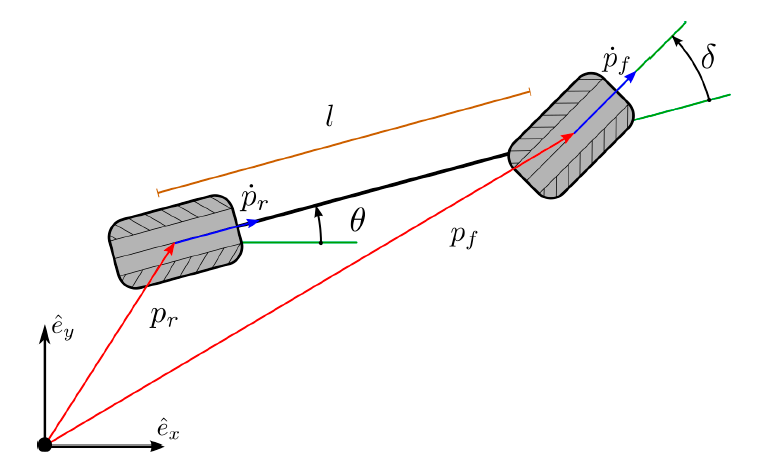
\includegraphics[width=13cm]{kinematics.png}
\caption{单轨道运动学模型图}
\caption*{$p_r$与$p_f$分别为后轮、前轮与地面的触点,$\theta$是车辆朝向角。$p_r$与$p_f$对时间的导数的方向受到非完整性约束的限制,如图中蓝色箭头所示。$\delta$是前轮导向角。}
\label{fig:kinematics}
\end{figure}

下面将对于包含朝向角$\theta$,点$p_r$的运动,点$p_f$的运动的坐标系导出差分约束。

为了满足接触点不滑动的约束,点$p_r$,$p_f$的运动必须与轮子的朝向共线,对后轮,该约束表示为
\begin{equation}
(\dot{p}_r\cdot \hat{e}_y)\cos(\theta)-(\dot{p}_r\cdot \hat{e}_x)\sin(\theta)=0,
\end{equation}
对前轮,有
\begin{equation}
(\dot{p}_f\cdot \hat{e}_y)\cos(\theta+\delta)-(\dot{p}_f\cdot \hat{e}_x)\sin(\theta+\delta)=0.
\end{equation}
该表达式通常被重写为关于基向量的分量形式。后轮运动在$\hat{e}_x$方向的分量为$x_r := p_r\cdot\hat{e}_x$,在$\hat{e}_y$方向为$y_r:=p_r\cdot \hat{e}_y$。前进速度为$v_r:=\dot{p}_r\cdot(p_f-p_r)/\|(p_f-p_r)\|$,即$\dot{p}_r$的模长乘上表示方向的符号。关于标量$x_r$,$y_r$和$\theta$,差分约束表示为
\begin{align}
\begin{split}
\dot{x}_r&= v_r\cos(\theta),\\
\dot{y}_r&= v_r\sin(\theta),\\
\dot{\theta}&=\frac{v_r}{l}\tan(\delta).
\end{split}
\end{align}
同样,对于点$p_f$的运动也具有差分约束
\begin{align}
\begin{split}
\dot{x}_f&= v_f\cos(\theta),\\
\dot{y}_f&= v_f\sin(\theta),\\
\dot{\theta}&=\frac{v_f}{l}\tan(\delta).
\end{split}
\label{eq:vf}
\end{align}
其中,前轮速度$v_f$与后轮速度有关系
\begin{equation}
\frac{v_r}{v_f}=\cos(\delta).
\end{equation}

对该车辆模型的规划和控制需要决定前轮导向角$\delta\in [\delta_{\min}, \delta_{\max}]$和前进速度$v_r\in [v_{\min}, v_{\max}]$。

一个常用的简化,如在[56]中用到的,是选择航向率$\omega$,而不是导向角$\delta$。二者存在关系
\begin{equation}
\delta=\arctan(\frac{l\omega}{v_r})
\end{equation}
这将朝向的运动简化为
\begin{equation}
\dot{\theta}=\omega, \quad \omega\in [\frac{v_r}{l}\tan(\delta_{\min}, \frac{v_r}{l}\tan(\delta_{\max})]
\end{equation}
这种模型有时被称为单轮车模型,因为它可以通过考虑单个车轮的运动而得出。

单轨道运动模型的一个重要变种是固定$v_r$的情况。 这有时被称为杜宾斯车,以莱斯特·杜宾斯(Lester Dubins)命名,他在规定切线的情形下得出了两点之间的最短时间运动[57]。另一个重要变种是Reed-Shepp车,当$v_r$取单值的正向和反向速度时,可以求出最小长度的路径[58]。 这两个模型已被证明对运动规划具有重要意义,并将在第四节进一步讨论。

运动学模型适用于低速情形,例如停车机动和城市驾驶。在该情形下车的惯性较小,不足以打破车轮不打滑的假设。该模型的主要缺点是它允许转向角度瞬间变化。如果运动计划模块要求产生这种瞬时变化,这将是有问题的。

转向角的连续性可以通过改进(\ref{eq:vf})来实现,其中转向角是转角速率的积分,如[49]所示。 方程式(\ref{eq:vf})变为
\begin{align}
\begin{split}
\dot{x}_f&= v_f\cos(\theta),\\
\dot{y}_f&= v_f\sin(\theta),\\
\dot{\theta}&=\frac{v_f}{l}\tan(\delta),\\
\dot{\delta}&=v_{\delta}.
\end{split}
\end{align}
除了对导向角的连续性限制,转角变化率也可以引入约束$v_{\delta}\in [\dot{\delta}_{\min},\dot{\delta}_{\max}]$。同样的问题也会出现在速度控制上。可以通过引入加速度保证速度控制的连续性。这种方法的缺点在于增加了模型的维数,将运动计划与控制问题变得更为复杂。

坐标系的选择不限于使用一个车轮位置作为位置坐标。 对于使用经典力学原理得出的模型,可以使用质心作为位置坐标,如[59],[60]或使用振荡中心,如[61],[62]。\\\\
\begin{center}
\textbf{原文索引}
\end{center}

\begin{translationbib}
\item Paden B, {\v{C}}{\'a}p M, Yong S Z, et~al.
\newblock A survey of motion planning and control techniques for self-driving
  urban vehicles\allowbreak[J].
\newblock IEEE Transactions on Intelligent Vehicles, 2016, 1\penalty0 (1):
  33--55.
\end{translationbib}